
%----------------------------------------------------------------------------------------
%	PACKAGES AND OTHER DOCUMENT CONFIGURATIONS
%----------------------------------------------------------------------------------------

\documentclass[11pt]{article} % Default font size is 12pt, it can be changed here

\usepackage{geometry} % Required to change the page size to A4
\geometry{a4paper, margin=2cm} % Set the page size to be A4 as opposed to the default US Letter

\usepackage{graphicx} % Required for including pictures

\usepackage{float} % Allows putting an [H] in \begin{figure} to specify the exact location of the figure

\usepackage{cite}

\begin{document}
	
	\title{Reading Project: Industrial Mathematics }
	\author{Margaret Duff }
	\date{Today}
	\maketitle
	
	\begin{abstract}
		Industrial Maths is.......
	\end{abstract}
	\tableofcontents 
	
	\section{Introduction}
	
	\section{Review of the International State of Industrial and Applied Mathematics, Mechanisms, Philosophy and Effectiveness}
	
	In this section we will look at the International State of Industrial and Applied Mathematics, Mechanisms, Philosophy and Applied Mathematics. This report will mainly be  focused on the UK but we will look elsewhere in the world for examples and comparisons. 
	
	We start by attempting to define Industrial Mathematics before questioning why it is important  and how it is done. Finally I will make some judgement of successes of Industrial Mathematics  and some of the challenges facing its future. Case studies will be discussed and referenced throughout to add provide concrete, real world references. 
	
	\subsection{Definitions} 
	
	Defining the language and descriptors of  Industrial Maths is not a simple task and indeed a variety of distinguished writers choose a range of definitions. 
	
	Even defining what it means to do Mathematical Research is fraught with complications. Even counting all those employed by universities and higher education institutes misses a large number of very talented mathematicians working elsewhere. 	Deloitte in their report 'Measuring the Economic Benefits of Mathematical Science Research in the UK' \cite{deloitteuk} count 'Mathematical Science Occupations' as those 'which either entail mathematical science research, or used mathematical science research-derived tools and techniques' a broad definition which includes individuals which may use mathematically derived techniques but have no understanding of the underlying mathematics, For example they includes all hospital and healthcare managers, social science researchers and public service administrative professionals, all very valuable jobs but not ones that I would put in the category of 'Mathematical Science Occupations'. 
	
	
	In a similar report Doloitte produced for the Dutch economy \ref{deloittedutch} they narrow this definition slightly by considering 'only people in jobs requiring a higher education' to be included.  A better but still quite broad definition and probably still includes healthcare managers and social science researchers!
	
	
	One might suggest considering only those people who currently use or research 'modern' mathematical science research tools, to avoid including all those people that use an excel spreadsheet to add up large numbers because "addition" is a mathematical technique. But then the definition of 'modern' is fraught: number theory developed during the end 19th and beginning of the 20th century underpins the very modern phenomenon of internet shopping. The radon transform, developed at the beginning of the 20th century, is behind most modern medical imaging. The motion of a rocket from the surface of the Earth to a landing on the Moon can be explained and described by physical principals discovered over 300 years ago by Sir Isaac Newton.
	
	
	For the purpose of this report, I  will consider Mathematics to be that which is of interest to academic mathematicians; it focuses  on the underlying structure and pattern of a problem and  looks for generalisations and derives exact or approximate solutions backed up by logical proof. The important clarification is that the application of well known techniques does not count. (Finally discounting those Social Scientists using statistical software!)
	
	
 Industry  I define it be any non-mathematical institution including: governments, businesses, manufacturers, other academic departments, hospitals, schools, charities etc. 


		A wealth of words are used as synonyms or colloquialisms for industrial mathematics: 'applicable', 'interdisciplinary, 'applied', 'knowledge transfer' or 'mathematics communication'. The Bond Report \cite{Bond} describes '\textit{Impactful Mathematics} as any mathematical method that has practical application and generates societal and/or economic value'. 
		
		For this report I will use the definition John Stockie describes in his essay 'Mathematics for Industry A personal Perspective' \cite{Stockie2015} that Industrial Mathematics includes: 
		
	\begin{itemize}
	\item mathematics that is done by non-academic mathematicians who work as employee of a company
	\item mathematics that is done by academic mathematicians within research institutions for a company, or in collaboration with a company
	\item mathematics that is inspired by industry and arise from an industrial setting. 
	\end{itemize}
	
	
	\subsection{Significance}
	
Although most people don't grow up to become mathematicians, they do grow up to rely on mathematics: from weather forecasts to smart phones; from the logisitcs of ensuring fresh food in supermarkets to online shopping or from the mechanics of a car engine to  the ability to understand the mysteries of the universe. Mathematicians like to tell you that "Maths is Everywhere" and indeed it is! 

However, a more quantitative argument is required to convince the most sceptical of readers. The Deloitte Report on the Economic benefits of mathematical research on the Uk economy \cite{deloitteuk} although perhaps over estimating, as discussed above, suggests that a total of 9.8million people are in employment attribute to mathematical science research, of which: 2.8 million can be directly attributed to mathematical science research, 2.9 million can be attributed indirectly through 'supply chain' impacts e.g. support staff, cleaners, technicians etc. and finally 4.1 million people have employment induced  through spending by households linked to mathematical science research. They also concluded that in 2010, mathematical science research in the UK generated direct gross-value added (GVA, value of the output less the value of the immediate consumption ) of approximately £208 billion, or around 16\% of total UK GVA.  Productivity, GVA per worker, in Mathematical Science occupations in 2010 was calculated at £74,000 per worker which can be compared to the UK productivity average in 2010 which was estimated to be £36,000 and the mean wage for mathematical science research jobs over £44,000. 
 
 These results evidence the significance of Mathematical Science Research on the UK economy and therefore how important that it continues to grow and remain competitive in the future. 
 
 
	
	SOMETHING ON THE Dutch Deloitte Report??
	
	 
	\subsection{Mechanisms}
	
	\subsubsection{In the UK  and in Europe }
	
	The Bond report \cite{Bond} found from its call for evidence a list of the most commonly cited examples of industrial mathematics mechanisms. This included: 
	\begin{itemize}
		\item \textit{Industrial Cooperative Awards in Science and Technology (CASE) PhD studentships }- A company allocated an award defines a research project and picks an academic partner. Once the arrangements for the project have been agreed between the company and research organisation, they can recruit a student. Students receive funding for a full EPSRC studentship for 4 years topped up by the company. A placement of at least 3 months at the company is required and projects should be in the area of engineering and the physical sciences. Students benefit from access training, facilities and expertise not available in an academic setting alone and academic partner institutions benefit from novel research collaborations and  development/ strengthening  of partnerships. Companies that were awarded EPSRC ICASE allocations for 2019/20 include the Defence Science and Technology Laboratory, Rolls-Royce PLc and the National Physical Laboratory. https://epsrc.ukri.org/skills/students/coll/icase/intro/
		
		\item \textit{Knowledge Transfer Network Ltd activities }- funded by innovate UK provides innovation network for other funders in line with its mission to drive UK growth. Examples of their programmes include: 
		\begin{itemize}
			\item \textit{ The 4manufacturing initiative } provides strategies for businesses to identify their barriers, challenges and next steps on the path to integrating modern technologies and systems to use digital data within both the business and the supply chain
			\item \textit{Knowledge transfer partnerships} (see below )
			\item \textit{Special Interest Groups} projects that focus our activity and accelerate innovation in cross-disciplinary topics of strategic importance. Groups funded included: Sustainable Aviation Fuel, Synthetic Biology, and Uncertainty Quantification and Management.
			\item \textit{The Access to Funding and Finance team} can help businesses understand and raise funding and finance – lending, grants, or equity based, as well helping prepare companies for investment.
		\end{itemize}
		\item \textit{Mathematics Study Groups} - Provide a forum for industrial scientists to work alongside academic mathematicians  on problems of direct industrial relevance. Initiated in Oxford in 1968 the format has been copied around the world and in even extending into other areas. The structure is as followed: 
		\begin{itemize}
			\item Approximately 80 mathematicians from a wide range of backgrounds
			\item On the first day the industrial representatives outline their project and aims
			\item The following few days are devoted to solving the problems. The industrial representatives are available to answer questions and guide the projects.
			\item On the last day, any progress made is presented
			\item Reports in the problems are produced after the meeting  
		\end{itemize}
		There are many benefits to industry including: 
		\begin{itemize}
			\item Access to the expertise of leading applied mathematicians to their problem
			\item New perspectives and fresh ideas on their problems
			\item Establishing links with research mathematicians
			\item An opportunity to formulate and reflect on problems  of long-term significance
		\end{itemize}	
		\item \textit{The Turing Gateway to Mathematics (TGM)} is the impact initiative of the Isaac Newton Institute (INI) based at the University of Cambridge. The TGM reaches out to and engages with the users of maths: industry, business, public sector and other scientific disciplines. Maintaining contacts across the world they can facilitate interactions and activities such as programmes of work, research and training events, as well as bespoke projects
		\item  \textit{A Knowledge Transfer Partnership} helps facilitate a 3 way partnership between a business or not for profit organisation, a research organisation or university and a graduate (known as the Associate). Designed for businesses who have an idea for a new project, capability or significant change but  do not have all the in-house expertise. Businesses benefit from new expertise and innovation. Research organisations benefit financially and  the possibility of publishing, identifying new research themes and apply their knowledge and expertise to real-world problems. Associates gain experience, often job opportunities and dedicated coaching, mentoring and personal development through working with the KTN.
		
	
	\end{itemize}

\paragraph{Incentives and Enablers} 
		See bond report 
		
	\subsubsection{Elsewhere in the world }	
PAGE 36 BOND REPORT - STATE IN GERMANY v. interesting 
		

	Smith institute
	
	Canadian examples - CQAM, Fields 
	
	\subsection{Successes}
	BOND Review 
	
	Women in industrial maths?? 
	\subsection{Challenges} 
	BOND Review
	
	\subsubsection{Identifying Suitable Problems and Creating links} 
	
	It can be hard for individual academics to know where to start, no recognised route, unsure of their own abilities 
	
	The Bond report quoted that 'just 26\% of SMES and large business respondents cited via a University knowledge/technology transfer office". Contacts seem to be based on a who-you-know sort of method; case studies commonly mention introductions at a "neighbourhood social event" \cite{Stockie2015}, NEED MORE EXAMPLES HERE... European successes in industrial mathematics????
	\subsubsection{Building working relationships}
	A long process!!!!
	Lack of understanding of business drivers and culture - different language/timescales/skillsets etc 
	Intellectual Property issues / complexity.inglexibility of contractual arrangment
	\subsubsection{Funding} 
	Talk about Bond Review and about 100 phd student places etc., boosting of EPSRC funding etc. 
	\subsubsection{Academic Career Paths} 
	Discussed heavily in the Bond Report: demand for mathematical experience is ever increasing especially in areas such as AI, machine learning, genomics, data science and finance. Skilled people can demand high salaries so academic departments need to change: to attract students they need to train individuals is these mathematical areas as well as in less traditional business and leadership skills and to attract academics they need to provide flexible, interesting  and remunerative career paths. 
	
	Free movement of skilled people between academia and industry is important to make and maintain links, build skills and create a supportive environment (LOOSE THAT THIRD ONE). 
	
	However time spent in industry is often seen as detrimental to an academic career progression, with its strong emphasis on sheer quantities of research publications and citations. 
	
	Academics often have many calls on their time and it is essential that adequate time, recognition and resources is available to enable and incentivise interaction with industry. Work done with industry must be recognised and rewarded by institutions. 
	
	Industrial mathematics is often time intensive with perhaps questionable clear rewards. Contacts take time to build and maintain and the time taken to do this is not generally recognised. Expected to do this on top of everything else. Funding for proof-of-concept/ sky blue thinking
	
	Bigger problem for early career researchers - short term post doc contracts etc etc   
	
	
	
	\subsubsection{Brexit}
	I am reluctant to mention the 'B' word but i think no report that looks at the future of Mathematical Research, Industry or Mathematics in Industry can avoid the topic. The whole scientific community is concerned over the future of funding and ability to collaborate (BREXIT LETTER NOBEL LAUREATES) and industry in the UK is facing an uncertain future (REFERENCE OR MORE HERE).
	
	I don't want to spend much time on this, but I would like to say that whatever happens, examples of success stories in industrial mathematics have demonstrated the need for collaboration: with industry, with other fields, with other departments and it will be vital for the continuing success of Industrial Mathematics that the spirit of collaboration is maintained. 
	
	\subsection{Case Study 1: Trip Wire Detection for Land Mines}
	
	The first case study that really stood out to me, was one brought to the second Industrial Problem-Solving Workshop (a Canadian version of the ESGI) held in Calgary in 1998. I follow an account of the project by one of the attendees, John Stockie \cite{Stockie2015} and the Study Group report \cite{Jessop}.
	
The industrial partner was ITRES Research LTD and they were experimenting mounting a detection camera on a boom ahead of a slowly moving truck which would look vertically downwards. It was hoped that an automatic algorithm would be used to find trip wires appearing in the image. 
	
	A report, the Landmine Monitor, produced in 1999 \cite{landmine} suggests that at the time the of the Study Group there were more than 250million Anti-personnel Mines in Stockpiles of which they were particularly concerned about remotely-delivered, surface laid anti vehicle mines that utilize trip wires which could explode from innocent acts by individuals. 
	
	A clearly defined  problem, that could have huge benefits worldwide so why was this a study group problem? Why hadn't a solution been implemented already? There were some inherent difficulties in detecting a tripwire including:
	\begin{itemize}
	\item wires are often partially covered by foliage
	\item wires are not uniform in illumination 
	\item wires are often purposefully camouflaged and come in a variety of colours and transparencies
	\item other image features may mimic lines such as vegetation 
	\item images are often noisy or blurry as trucks and cameras move or the camera fails to focus. Natural elements also cause additional artefacts in the field of view
	\end{itemize}
	The goal of the week long study group was to have a first attempt at developing an algorithm that was \textsl{robust} enough to cope with the problems above; \textit{reliable }enough to detect trip wires in with near perfect sensitivity and a high specificity and to be \textit{fast} enough to run before the truck detonates a landmine. 
	
	We will look at 3 elements of their work: pre-processing, line detection and improving speed:
	\paragraph{Pre-processing}
\begin{itemize}
	\item \textbf{Laplacian Filter}: Mathematicians love definitions and in this case careful consideration of the definition of a wire in an image indicates a possible direction of work. Defining image intensity to be a function $u(x,y)$ of position $(x,y)$ and thus a line, a sharp edge, is one in which the function $u(x,y) $ has a high curvature.
	To enhance this feature the convolution of the image with a Laplacian filter is taken. This has a similar effect to taking the second derivative and accentuates regions of high curvature.	
	\item \textbf{Edge detection }: Edges are then found in the filtered image using either the Sobel edge detector or the log method. The result is a binary image with found edges indicated. 
	\end{itemize}
	
	\paragraph{Line Detection}
	Continuing the theme of precise definitions: the differentiating factor between any old line and a potential trip wire is that a wire is locally straight and although could be partially hidden consists of a sequence of co-linear line segments. In order to detect such lines they use: 
		\begin{itemize}
		\item \textbf{Radon Transform}: The Radon transform of a 2D image given by:
		
		\begin{equation}
			R(\rho, \theta)=\int_{R^2} u(x,y)\delta(x\cos(\theta)+y\sin(\theta)-\rho) dx dy 					
		\end{equation}
		transforming the image from an $(x,y) $ domain to a $ (\rho, \theta)$ domain. Peaks in the $ (\rho, \theta)$ domain correspond to lines of the form $ x\cos(\theta)+y\sin(\theta)=\rho$ in the $(x,y) $ domain. 
		\item \textbf{Threshold transformed images }: Finding the peaks in the $ (\rho, \theta)$ domain requires some sort of threshold. If the threshold is too high then no wires are found, too low and there are too many false positives. What is defined as a wire is independent of individual images but variations in images can cause additional noise inflating all the values in the $ (\rho, \theta)$ domain causing issues. This is not a simple issue. 
	\end{itemize}
	\paragraph{Algorithm Speed}
		\begin{itemize}
		\item \textbf{Using the FFT}: A the time of the Study Group Matlab's inbuilt Radon transform did not take advantage of the fast Fourier transform to speed up implementation. Such a possibility was discussed. 
		\item \textbf{Exploiting the method of image acquisition}: Images are received from the camera as a sequence of lines that are constantly updated. Discussion was had as to how the intensities in the $ (\rho, \theta)$ domain can be continuously updated as each new line is attained, reducing the number of computations compared to repeatedly taking the radon transform of the whole image. 
	\end{itemize}
	
	The algorithm produced during the week was in no way perfect, struggling with some of the more 'difficult' images and ones where the wires were oblique. Results were presented to the industry partner but future collaboration was not forthcoming, a shame but potentially due to the military applications of such work. There is evidence that ITRES continued working on this problem with conference proceedings released in 2000 \cite{Babey}. \emph{TO READ THIS PLEASE!!!!!!!!}
	

	
	
	\subsection{Case Study 2 - Shelter: Homeless Populations}
	
To READ https://www.gov.scot/binaries/content/documents/govscot/publications/research-publication/2018/06/health-homelessness-scotland/documents/00536908-pdf/00536908-pdf/govscot\%3Adocument
	
   Brought to ESGI 29, held in Oxford in March 1996 a problem from the charity Shelter to model the numbers of homeless and non-homeless people in a Borough. The model should then be able to predict changes in homeless populations as a result in changes of local policy. I follow the report produced at the end of the study group \cite{Shelter1996}
	
	The populations was split into broad classes: 
	\begin{itemize}
		\item $ T= $ N umber of households in temporary accommodation (Homeless)
		\item $  P= $ Number of households permanently resident in council housing stock
		\item $ G= $ Number of households in private sector accommodation 
	\end{itemize}
	This is then further subdivided as:
	\begin{itemize}
		\item $ P_R= $ Number of households in council stock and not  seeking transfer to other council housing stock 
		\item $ P_N= $ Number of households in council stock and seeking transfer 
		\item $ G_R= $ Number of households in private sector accommodation seeking transfer to council housing stock 
		\item $ G_N= $ Number of households in private sector accommodation and not seeking transfer
	\end{itemize}

Hence we have the following relations 
\begin{itemize}
	\item $ P=P_R+P_N $
	\item $ G=G_R+G_N $
	
\end{itemize}

Also define: 
\begin{itemize}
	\item Number of Households on the register,$  R=T+P_R+G_R $
	\item $ P_0 = $ Total availability of housing stock 
	\item $ G_0= $ Total number of households in the Borough
\end{itemize}

The flows in and out of population groups are shown in Figure \ref{fig:homelessrates}. A few assumptions about negligible flows have been assumed to simplify the problem: it is assumed that homeless families only come form the private sector and also that flows from $ G_R $ to $ G_N $ and $ T $ back to $ G $ are negligible. 

This gives a system of differential equations
\begin{eqnarray}
\frac{dG_N}{dt}=-k_5 G_N-k_3 G_n +k_6 P\\
\frac{dG_R}{dt}=-k_5 G_R +k_3 G_N -k_4 (P_0-P)G_R\\
\frac{dT}{dt}=k_5 G -k_1(P_0 -P)T\\
\frac{dP_N}{dt}=-k_6 P_N -k_7 P_N +(P_0-P)(k_4 G_R +k_1 T+k_8 P_R)\\
\frac{dP_R}{dt}=-k_6 P_R+k_7 P_N -k_8(P_0-P)P_R
\end{eqnarray}
	 \begin{figure}
	 	\centering
	 	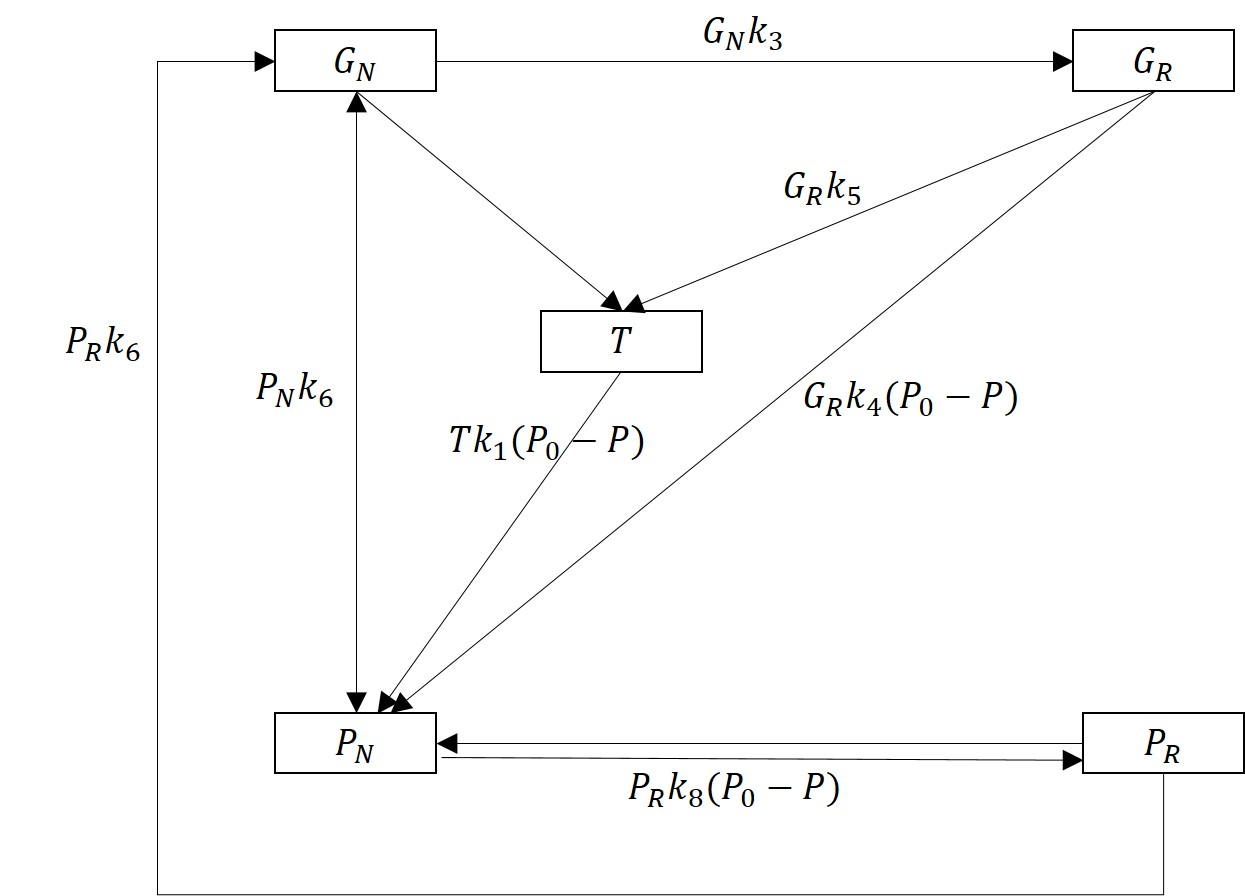
\includegraphics[width=0.7\linewidth]{Report_images/homeless_rates}
	 	
	 	\caption{A diagram to show  flows and and associated rates of households moving  between population groups}
	 	\label{fig:homelessrates}
	 \end{figure}
	 
	These equations implicitly assume that:  
	\begin{itemize}
		\item Birth and death rates can be neglected
		\item No migration in and out of the borough 
		\item Rates depend only on the present circumstances there is no delay e.g. due to administrative processes 
	\end{itemize}

These equations look intractable but substituting $ G_0=P+T+G_r+G_N $ and $ G_0=G+P+T$ reduces the system to 3 differential equations:

\begin{eqnarray}
\frac{dT}{dt}=k_5 G -k_1(P_0 -P)T\\
\frac{dG_R}{dt}=-k_5 G_R+k_3(G_0-P-T-G_R)-k_4(P_0-P)G_R\\
\frac{dP}{dt}=-k_6P+(P_0-P)(k_4G_R+k_1T)
\end{eqnarray}
	
	They looked for equilibrium solutions, so setting the left hand side of the equations to zero. They were able to see that a feasible equilibrium solution always exists, where the number of occupied council houses is positive but no greater than the number actually available. 
	
	Looking for analytic solutions of the equations in full generality was deemed unproductive for the short intensive time available in a Study group so focus was moved to looking for numerical solutions. 
	
	Initial values were chosen to represent a typical metropolitan borough. calculations were carried out with numbers of people rather than families. They found that the steady state solution was locally stable but that the values showed high sensitivity from the initial data and values. Thus generalised discussion about results for the "typical" borough or for all boroughs is not possible. They did however manage to make some useful inferences: 
	

	\begin{itemize}
		\item The populations only settle down to the steady state values over a period of about 30 years. This is a much larger time frame than changes in local and national policies and is large enough that births, deaths and migration should be taken into account. Future work should either aim to increase the complexity of the model to take this into account or should look closer at the initial dynamics and variation. 
		\item Reducing the constant $ k_1 $ by a factor of 10, signifying a change in policy so that much less priority is giving to the homeless on council waiting lists causes very little change apart from a 10-fold increase in the numbers of homeless in the borough. The amount of vacant council property increased a little but not sufficiently to cope with the increase in homeless families. The factor $ k_1 $ is important. 
	\end{itemize}
	
	The work was continued after the study group, including a paper produced based mainly on the work done during the study group \cite{Byatt-Smith2003}. The work was also continued as the MSc project and then the PhD project of Andrew Waugh, supervised by one of the study group attendees Andrew Lacey, at Herriot Watt University. 
	
	We look at one of the extensions he made to the Study Group Model in the form of a points based model \cite{Waugh1999}. This aims to model the mechanisms used to allocate houses to those on the waiting list. 
	
	
	
	\subsection{Case Study 3: Optimisation of the “118” Emergency Management System in Milan  }
	The book "European Success Stories in Industrial Mathematics" \ref{Lery2011} contains a wealth of great examples of effective knowledge transfer and collaboration. One particular example, "Optimisation of the "118" Emergency Management System in Milan" attracted me because of its real-world importance and clear mathematical optimisation problem but also because of a particular sentence: 
	
	\begin{quote}
		''In spite of being developed by academic personnel, the outcome of the project has been actually implemented''
	\end{quote}

	Perhaps, not a sentence I should have taken out of context, but CONTINUE HERE 
	
	

	I follow the 2013 paper by R. Arinhieri, G. Carello and D. Morale \cite{Aringhieri2016}  to describe some fo the work behind this case study.
	
	They focused on 3 areas: evaluation of the current EMS system; study of operational policies which can improve the system performance through a simulation model and using optimisation to fund an alternative set of ambulance posts. 
	\begin{figure}
		\centering
		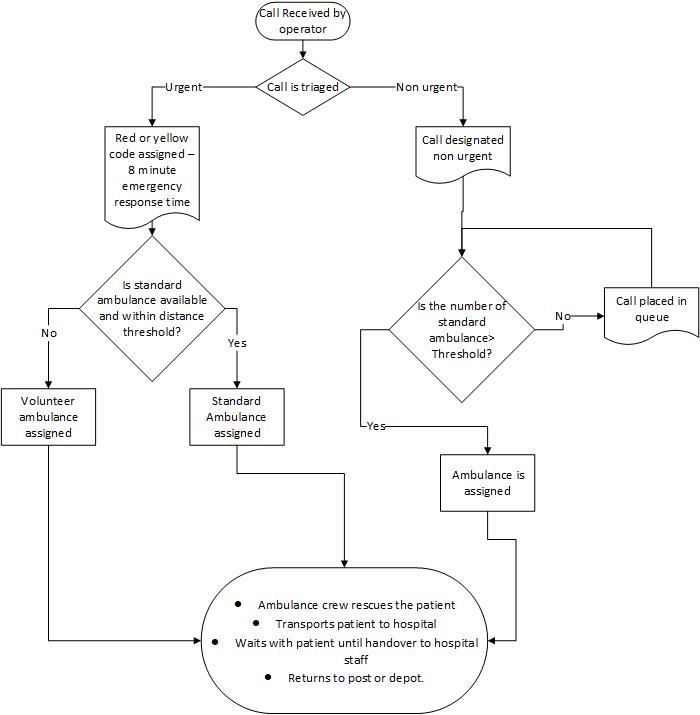
\includegraphics[width=0.9\linewidth]{Report_images/MilanEMS}
		\caption{The process of responding to an emergency call}
		\label{fig:milanems}
	\end{figure}
\paragraph{Evaluation of the current EMS system }
	Figure \ref{fig:milanems} documents  the process of responding to an emergency call. A few points to highlight: 
	\begin{itemize}
		\item Italian law states that urgent calls have to be responded to in 8 minutes in urban areas. This threshold is also a major measure of performance 
		\item The Milano EMS used two types of ambulance: 
		\begin{itemize}
			\item Standard/prepaid ambulances - a set composed of 29 ambulances that are always available. They represent a fixed cost regardless of the number of missions performed. Ambulances are located at ambulance posts ready to be deployed.
			\item "Volunteer" ambulances - run by various volunteer organisations who own them. They can be summoned if needed and the cost is per mission. They are based at their organisation's head quarters.
		\end{itemize}
		The focus of the work was on the first set: to try and serve the majority of the requests with standard ambulances in order to reduce costs and ensure consistency of quality of care. 
		\item After the ambulance has been assigned to the point were it returns to its post or depot after completing a mission the ambulance is unavailable and cannot be diverted. 
	\end{itemize}
\paragraph{Development of a simulation model in order to test operational policies }
Analysis of the historical data found that there was room for improvement- on average 60.1\% of the urgent calls meet the 8 minute response time with a 95\% confidence interval of $ [56.13\%, 64.06\%] $. Any investment in infrastructure to try and improve these figures would be expensive and with no guarantee of success: a mathematical model could help test different scenarios. 

In the model ambulance locations are plotted on a map of Milan at each point in time, the speed assigned to each ambulance is a function of the time of the day and the area in which the ambulance is currently located. This is more  computationally intensive compared to an event based model where the movement of tan ambulance from a place to another one is usually represented by an new event, the actual movement of the ambulance is not a part of simulation model.The model focused on just the set of standard ambulances.

Each emergency request was generated by using real data of a given day, a variety of days were selected to test the model, including some selected critical days which could be representative of emergency scenarios. 

The model was initialised to model current procedure and for the 7 days worth of events used, the model predicted a that 63.92\% of the urgent calls would be responded to within the 8minute deadline. This is within the 95\% confidence interval produced from historical data and suggests the simulation is representative of actual EMS behaviour. 

Various parameters could now be varied in order to test different improvement strategies:
\begin{itemize}
	\item \textbf{Increases to  ambulance average speed}: Road improvements, reserved lanes and systems to wave ambulances through traffic lights could all increase average ambulance speed. An average increase of 5km/h was shown in the model to increase the number of urgent calls reached within 8minutes by approximately 20\%.
	\item \textbf{Adding a new ambulance}:  Adding a new standard ambulance to the fleet would be an expensive investment and the model showed that with the current set of ambulance posts that there would be little improvement in response rates, due to ambulances gathering in a few posts and leading to unbalanced global coverage. 
	\item \textbf{Moving to "smart" ambulances}: The possibility of summoning an ambulance before it reaches its post on return from a mission, or in redirecting an ambulance on its way to a less urgent mission can be evaluated using the model, because of the agent based approach to modelling ambulances. At the time of the work, ambulances were not equipped with GPS systems and therefore this sort of assignment was not possible. On the heaviest days the model was predicting up to a 20\% improvement in the number of urgent calls responded to within the 8 minute deadline, similar figures to that of increases in ambulance speed but at potentially a much reduced cost and less dependent on external factors such as weather. 
\end{itemize}

\paragraph{Finding an alternative set of ambulance posts}
HELP!!!! NEEDS MORE OF MY OWN INTUITION 

Low Priority Calls Coverage (LPCC) optimisation model was developed by the authors to take a potential set of posts and solve a minimisation problem, to discover the theoretical minimum number of required ambulances and where their posts should be located. First some definitions of variables:
\begin{itemize}
	\item $V=$ the set of points to be covered. For each point $ i \in V $, $d_i^h$ denotes the amount of hight priority demands and $d_i^l$ low priority demands 
	\item $ W= $ the set of candidate post locations. The capacity associated to each post is denoted by $ k_j $.
	\item Let $ W_i^h $ be the set of candidate posts from which a demand point $ i $ can be reached within the 8 minute threshold. 
	We introduce a second time limit in which a certain percentage of non urgent calls must be seen, and similarly let $ W_i^l $ be the set of posts from which $ i $ can be reached in this longer time frame
	\item Let $ y_{ij} $ be the fraction of emergency demand of point $ i  $ served by an ambulance at post $ j $. Similarly $ w_{ij} $ to be the fraction of non urgent demand at point $ i  $ served by an ambulance at point $ j $.
	\item An integer variable $ x_j $ is define for each post $ j $, representing the number of ambulances assigned to the post, this can be zero.
\end{itemize}

\begin{eqnarray}
\min \ z=\sum_{j\in W} x_j \label{1a}\\
s.t.\ &\sum_{j\in W_i^h} x_j\geq1\ \ &\forall i \in V\label{1b}\\
&\sum_{j\in W_i^h} y_{ij}=1\ \ &\forall i \in V\label{1c}\\
&\sum_{j\in W}w_{ij}=1 \ \ & \forall i\in V \label{1d}\\
&\sum_{i \in V} \sum_{j \in W_i^l} d_i^l w_{ij} \geq q \sum_{i \in V} d_i^l\label{1e}\\
&\sum_{i \in V} (d_i^h y_{ij} +d_i^l w_{ij}) \leq k_jx_j & \forall j \in W\label{1f}\\
&x_j\in Z_+, \ w_{ij} \in [0,1], \ &\forall i \in V,\  \forall j \in W \label{1g}
\end{eqnarray}
Where Eq \ref{1a} is the objective function: to minimise the number of required ambulances. Eq \ref{1b} ensures that there is coverage over all the city. Eq \ref{1c} ensures that urgent calls are served within the given time limit. Eq \ref{1d} guarantees that all the low priority calls can be served by and ambulance at any posts. Eq \ref{1e} forces that a given percentage of the non-urgent calls ate served with a second time limit. Eq \ref{1f} limits the number of missions in a given time frames. Finally \ref{1g} defines the domains of the variables 
 
 
For the solution of Milan the city was divided into 493 grid squares, chosen such that the area in each gird is covered by the same set of candidate post locations. Thus as long as each sub area is covered, all possible areas will also be covered. They set $ V=W $, $ q=0.5 $ and the non-urgent time frame to be 30minutes. This gives an optimal solution of 25 ambulances.

The remaining 4 ambulances are then allocated using an iterative procedure where the model from the previous section is used, and ambulance posts given  a ranking determining their utilisation. New posts are added in such a way as to decrease the highest utilisation value , this is iterated until there is a post located for each ambulance. 

This could also be used to design a set of posts to reach a threshold level of performance
	\subsection{Case Study 4: Mathematical Modelling of the Dynamics of Meningococcal Meningitis in Africa  }
The book "UK Success stories in Industrial Mathematics" \cite{Aston2016} is a collection of cases studies selected from those Impact Case Studies submitted to the 2014 Research Excellence Framework. They are seen as shining examples of the mathematical sciences community engaging with problems and organisations outside of academia. 36 problems were selected out of the 250 submitted for the REF and I aimed to pick just one to write up as a case study- a challenge indeed!


The African meningitis belt spans sub Saharan Africa and see periodic fluctuations of meningococcal meningitis, cases appearing every dry season, drop off over the rainy season and a major epidemic emerges every 6-14years. Across the world, meningitis causes about 135,000 deaths annually and substantial data is available across the African meningitis belt, so mathematical modelling of epidemiology of meningococcal meningitis could lead to substantial benefits. Indeed, modelling has been attempted by a number of groups but we follow the work by K.B.Blyuss at the University of Sussex described in "UK Success stories in Industrial Mathematics." and the associated paper \cite{Irving2012}.


\paragraph{Initial Modelling and Identification of Reproduction Number  }
Looking for a simple model the team looked towards the standard SIR model. In the case of meningitis, individuals can be carriers without developing the infection and there is a high ratio of carriers to cases, thus an additional "carrier" class was a necessary addition, giving 4 classes: 
\begin{itemize}
	\item S= Susceptible
	\item C=Carriers
	\item I=Infected
	\item R=Recovered
\end{itemize}
The total population is $ N=S+C+I+R $. The question of temporary immunity was a major part of this work and they considered a variety of models where there was:
\begin{itemize}
	\item no immunity, and thus no recovered class, recovered individuals went straight  to susceptible 
	\item   immunity only if they have had developed a meningitis infection, if individuals had only been a carrier then they got new immunity
	\item immunity if they had been a carrier, developed the infection or both
\end{itemize}

\begin{figure}
	\centering
	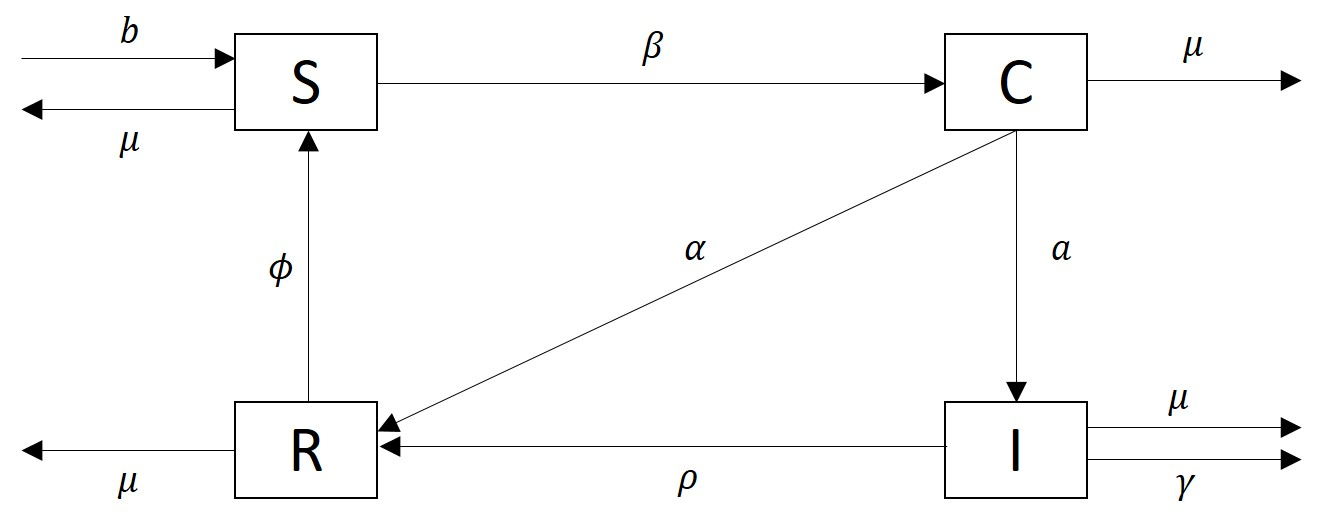
\includegraphics[width=0.7\linewidth]{Report_images/meningitis_model}
	\caption{A diagram to show the flows between population groups in the chosen meningitus model, taken from Fig 2 in paper  \cite{Irving2012}}
	\label{fig:meningitismodel}
\end{figure}



 Modelling all 3 cases they found the best fit to the observed data was the last case and the model shown in Figure \ref{fig:meningitismodel}, with rates defined as followed:
\begin{itemize}
	\item $ \beta =$ the transmission rate
	\item $ a= $ the rate at which carriers develop an invasive disease
	\item $ \alpha =$ the rate at which carriers recover 
	\item $ \rho= $ the rate at which individuals with invasive disease recover
	\item $ \phi = $ the rate at which recovered individuals loose their immunity becoming susceptible again 
	\item $ \mu = $ natural death rate
	\item $ \gamma = $ disease induced death rate

\end{itemize}

The birth rate is chosen to be $ b=\mu N +\gamma I  $ so that the total population $ N=S+C+I+R $ is constant. This assumption is only suitable for relatively short term modelling before the assumptions break down but it is a good starting point and gives equations: 

\begin{eqnarray}
	\frac{dS}{dt}= b +\phi R-\beta \frac{S(C+I)}{N}-\mu S\\
	\frac{dC}{dt}=\beta \frac{S(C+I)}{N}-(a+\alpha+\mu)C\\
	\frac{dI}{dt}=aC-(\rho +\gamma+\mu)I\\
	\frac{dR}{dt}=\rho I +\alpha C-(\phi+\mu)R
\end{eqnarray}
	
	Which under rescaling by $ N $ and using  $ I=S+C+I+R $ to remove $ S $ from the equations gives
	\begin{eqnarray}
	\dot{C}=\beta(1-C-I-R)(C+I)-(a+\alpha+\mu)C\\
	\dot{I}=aC-(\rho+\gamma+\mu)I\\
	\dot{R}=\rho I+\alpha C-(\phi+\mu)R
	\end{eqnarray}
	
	We look for steady state solutions when $ \dot{C}=\dot{I}=\dot{R}=0 $. Messy calculations but one finds:
	\begin{eqnarray}
	C^*=\lambda (\phi+\mu)(\rho+\gamma+\mu)\\
	I^*=\lambda a(\phi+\mu)\\
	R^*=\lambda(\alpha(\rho+\gamma+\mu)+\rho\alpha)
	\end{eqnarray}
	
	Where $ \lambda $ is a proportionality constant that can be found by subbing into $  \dot{C}=0 $ giving $ \lambda=0 $ or:
	
	\begin{eqnarray}
	\lambda=\frac{\beta(\gamma+\rho+\mu+a)-(\gamma+\rho+\mu)(\alpha+a+\mu)}{\beta(\rho+\mu+a)[(\rho+\gamma+\mu)(\phi+\mu+\alpha)+a(\phi+\mu+\rho)]}\\
	=\frac{(\rho+\gamma+\mu)(a+\alpha+\mu)}{\beta(\rho+\mu+a)[(\rho+\gamma+\mu)(\phi+\mu+\alpha)+a(\phi+\mu+\rho)]}\frac{\beta(\gamma+\rho+\mu+a)-(\gamma+\rho+\mu)(\alpha+a+\mu)}{(\rho+\gamma+\mu)(a+\alpha+\mu)}\\
	=\frac{(\rho+\gamma+\mu)(a+\alpha+\mu)}{\beta(\rho+\mu+a)[(\rho+\gamma+\mu)(\phi+\mu+\alpha)+a(\phi+\mu+\rho)]}\left( \frac{\beta(\gamma+\rho+\mu+a)}{(\rho+\gamma+\mu)(a+\alpha+\mu)}-1\right) 
	\end{eqnarray}
	
	
	An important quantity to identify when looking at epidemiology models is the reproduction number,  $  R_0 $. As defined in \cite{VanDenDriessche} it is such that if $ R_0 < 1 $, then the disease free  steady state $ (C,I,R)=(0,0,0) $ is stable, and the disease cannot invade the population, but if $  R_0 > 1 $, the disease free steady-state is unstable and an epidemic can take hold. 
	For $ R_0>1 $ a new stable stationary point should exist for values of $ C,I,R>0 $.
	In our case looking at our two potential steady states and the equations for $\lambda$ we find that in order for $C^*, I^*, R^*>0$ we require: 
	
	\begin{eqnarray}
	R_0=\frac{\beta(\gamma+\rho+\mu+a)}{(\gamma+\rho+\mu)(a+\alpha+\mu )}>1
	\end{eqnarray}
	Giving us the reproduction number and valuable information about in which circumstances meningitis will spread or be contained. 
	
Again using \cite{VanDenDriessche}  a more qualitative description fo the reproduction number is  the number of new infections produced by a typical infective individual in a population at a disease free steady state.  If $ R_0 < 1 $, then on average an infected individual produces less than one new infected	individual over the course of its infectious period, and the infection cannot grow. Conversely, if 	$ R_0 > 1 $, then each infected individual produces, on average, more than one new infection, and the disease can invade the population. 


We consider adding a new carrier to an otherwise healthy population. Two things can happen, the carrier can directly infect healthy members of the population or the carrier can become infected and then infect healthy members of the population. 

The expected amount of time the carrier remains a carrier is
 \begin{eqnarray}
\frac{1}{a+\alpha+\mu}
\end{eqnarray}
and as a carrier they infect members of the general population at rate $ \beta $ giving expected number of people infected by a single carrier that doesn't become infected is:
 \begin{eqnarray}
\frac{\beta}{a+\alpha+\mu}
\end{eqnarray}

The carrier becomes infected with probability 
 \begin{eqnarray}
\frac{a}{a+\alpha+\mu}
\end{eqnarray}
calculated from the expect time the carrier remains a carrier multiplied by the rate of contracting the infection. The expected time they remain infected is: 
 \begin{eqnarray}
\frac{1}{\rho+\delta+\mu }
\end{eqnarray}
and they infect healthy individuals with rate $\beta  $

Thus the expected number of new cases is: 

\begin{eqnarray}
R_0=\frac{\beta}{a+\alpha+\mu}+\frac{a}{a+\alpha+\mu}\frac{\beta}{\rho+\delta+\mu }\\
=\frac{\beta(\gamma+\rho+\mu+a)}{(\gamma+\rho+\mu)(a+\alpha+\mu )}
\end{eqnarray}
Matching the result from before.

\paragraph{Adding the seasonal effects  }


To try and explain the seasonal variations in the number of cases, they introduced a seasonally varying rate of disease transmission:
\begin{eqnarray}
\beta(t)=\beta_0(1+\epsilon_\beta \cos(2\pi t))
\end{eqnarray}
	
The model then exhibits a wide variety of dynamical behaviours and importantly, sees chaotic behaviour for a range of values of $\phi$ which is significant as $\frac{1}{\phi}$ is the expected duration of temporary immunity. Simulations suggest that that the model is able to produce the regular annual epidemics as well as epidemics with larger periods, can produce different amplitudes of epidemics and chaotic behaviour such as which is seen in the data. The longer inter epidemic periods, such as the 6-14years seen in the data corresponds to $\frac{1}{\phi}\approx 2 $ years.  
\paragraph{Impact}

\begin{itemize}
	\item The model highlighted the important role of the temporary immunity and the value of the constant $\phi$. A focus on computing an accurate value for this constant or working clinically to alter its value could be hugely beneficial
	\item An accurate value of the reproduction rate, $ R_0 $ is important when optimising vaccination deployment, reducing costs and increasing effectiveness. 
	\item Future work could look at including spatial effects, potentially including satellite and meteorological data. An advance disease warning system, for the larger deadlier outbreaks every 6-14 years would be hugely beneficial. 
\end{itemize}
	
	\section{Real Case Study}
	
	\section{Final Thoughts} 

	
	\bibliography{Industrial_Reading_Project}
	\bibliographystyle{plain}
\end{document}